\documentclass{ximera}  


%\usepackage{todonotes}
%\usepackage{mathtools} %% Required for wide table Curl and Greens
%\usepackage{cuted} %% Required for wide table Curl and Greens
\newcommand{\todo}{}

\usepackage{esint} % for \oiint
\ifxake%%https://math.meta.stackexchange.com/questions/9973/how-do-you-render-a-closed-surface-double-integral
\renewcommand{\oiint}{{\large\bigcirc}\kern-1.56em\iint}
\fi


\graphicspath{
  {./}
  {jpg}
  {ximeraTutorial/}
  {basicPhilosophy/}
  {functionsOfSeveralVariables/}
  {normalVectors/}
  {lagrangeMultipliers/}
  {vectorFields/}
  {greensTheorem/}
  {shapeOfThingsToCome/}
  {dotProducts/}
  {partialDerivativesAndTheGradientVector/}
  {../productAndQuotientRules/exercises/}
  {../motionAndPathsInSpace/exercises/}
  {../normalVectors/exercisesParametricPlots/}
  {../continuityOfFunctionsOfSeveralVariables/exercises/}
  {../partialDerivativesAndTheGradientVector/exercises/}
  {../directionalDerivativeAndChainRule/exercises/}
  {../commonCoordinates/exercisesCylindricalCoordinates/}
  {../commonCoordinates/exercisesSphericalCoordinates/}
  {../greensTheorem/exercisesCurlAndLineIntegrals/}
  {../greensTheorem/exercisesDivergenceAndLineIntegrals/}
  {../shapeOfThingsToCome/exercisesDivergenceTheorem/}
  {../greensTheorem/}
  {../shapeOfThingsToCome/}
  {../separableDifferentialEquations/exercises/}
  {vectorFields/}
}

\newcommand{\mooculus}{\textsf{\textbf{MOOC}\textnormal{\textsf{ULUS}}}}

\usepackage{tkz-euclide}\usepackage{tikz}
\usepackage{tikz-cd}
\usetikzlibrary{arrows}
\tikzset{>=stealth,commutative diagrams/.cd,
  arrow style=tikz,diagrams={>=stealth}} %% cool arrow head
\tikzset{shorten <>/.style={ shorten >=#1, shorten <=#1 } } %% allows shorter vectors

\usetikzlibrary{backgrounds} %% for boxes around graphs
\usetikzlibrary{shapes,positioning}  %% Clouds and stars
\usetikzlibrary{matrix} %% for matrix
\usepgfplotslibrary{polar} %% for polar plots
\usepgfplotslibrary{fillbetween} %% to shade area between curves in TikZ
\usetkzobj{all}
\usepackage[makeroom]{cancel} %% for strike outs
%\usepackage{mathtools} %% for pretty underbrace % Breaks Ximera
%\usepackage{multicol}
\usepackage{pgffor} %% required for integral for loops



%% http://tex.stackexchange.com/questions/66490/drawing-a-tikz-arc-specifying-the-center
%% Draws beach ball
\tikzset{pics/carc/.style args={#1:#2:#3}{code={\draw[pic actions] (#1:#3) arc(#1:#2:#3);}}}



\usepackage{array}
\setlength{\extrarowheight}{+.1cm}
\newdimen\digitwidth
\settowidth\digitwidth{9}
\def\divrule#1#2{
\noalign{\moveright#1\digitwidth
\vbox{\hrule width#2\digitwidth}}}





\newcommand{\RR}{\mathbb R}
\newcommand{\R}{\mathbb R}
\newcommand{\N}{\mathbb N}
\newcommand{\Z}{\mathbb Z}

\newcommand{\sagemath}{\textsf{SageMath}}


%\renewcommand{\d}{\,d\!}
\renewcommand{\d}{\mathop{}\!d}
\newcommand{\dd}[2][]{\frac{\d #1}{\d #2}}
\newcommand{\pp}[2][]{\frac{\partial #1}{\partial #2}}
\renewcommand{\l}{\ell}
\newcommand{\ddx}{\frac{d}{\d x}}

\newcommand{\zeroOverZero}{\ensuremath{\boldsymbol{\tfrac{0}{0}}}}
\newcommand{\inftyOverInfty}{\ensuremath{\boldsymbol{\tfrac{\infty}{\infty}}}}
\newcommand{\zeroOverInfty}{\ensuremath{\boldsymbol{\tfrac{0}{\infty}}}}
\newcommand{\zeroTimesInfty}{\ensuremath{\small\boldsymbol{0\cdot \infty}}}
\newcommand{\inftyMinusInfty}{\ensuremath{\small\boldsymbol{\infty - \infty}}}
\newcommand{\oneToInfty}{\ensuremath{\boldsymbol{1^\infty}}}
\newcommand{\zeroToZero}{\ensuremath{\boldsymbol{0^0}}}
\newcommand{\inftyToZero}{\ensuremath{\boldsymbol{\infty^0}}}



\newcommand{\numOverZero}{\ensuremath{\boldsymbol{\tfrac{\#}{0}}}}
\newcommand{\dfn}{\textbf}
%\newcommand{\unit}{\,\mathrm}
\newcommand{\unit}{\mathop{}\!\mathrm}
\newcommand{\eval}[1]{\bigg[ #1 \bigg]}
\newcommand{\seq}[1]{\left( #1 \right)}
\renewcommand{\epsilon}{\varepsilon}
\renewcommand{\phi}{\varphi}


\renewcommand{\iff}{\Leftrightarrow}

\DeclareMathOperator{\arccot}{arccot}
\DeclareMathOperator{\arcsec}{arcsec}
\DeclareMathOperator{\arccsc}{arccsc}
\DeclareMathOperator{\si}{Si}
\DeclareMathOperator{\scal}{scal}
\DeclareMathOperator{\sign}{sign}


%% \newcommand{\tightoverset}[2]{% for arrow vec
%%   \mathop{#2}\limits^{\vbox to -.5ex{\kern-0.75ex\hbox{$#1$}\vss}}}
\newcommand{\arrowvec}[1]{{\overset{\rightharpoonup}{#1}}}
%\renewcommand{\vec}[1]{\arrowvec{\mathbf{#1}}}
\renewcommand{\vec}[1]{{\overset{\boldsymbol{\rightharpoonup}}{\mathbf{#1}}}\hspace{0in}}

\newcommand{\point}[1]{\left(#1\right)} %this allows \vector{ to be changed to \vector{ with a quick find and replace
\newcommand{\pt}[1]{\mathbf{#1}} %this allows \vec{ to be changed to \vec{ with a quick find and replace
\newcommand{\Lim}[2]{\lim_{\point{#1} \to \point{#2}}} %Bart, I changed this to point since I want to use it.  It runs through both of the exercise and exerciseE files in limits section, which is why it was in each document to start with.

\DeclareMathOperator{\proj}{\mathbf{proj}}
\newcommand{\veci}{{\boldsymbol{\hat{\imath}}}}
\newcommand{\vecj}{{\boldsymbol{\hat{\jmath}}}}
\newcommand{\veck}{{\boldsymbol{\hat{k}}}}
\newcommand{\vecl}{\vec{\boldsymbol{\l}}}
\newcommand{\uvec}[1]{\mathbf{\hat{#1}}}
\newcommand{\utan}{\mathbf{\hat{t}}}
\newcommand{\unormal}{\mathbf{\hat{n}}}
\newcommand{\ubinormal}{\mathbf{\hat{b}}}

\newcommand{\dotp}{\bullet}
\newcommand{\cross}{\boldsymbol\times}
\newcommand{\grad}{\boldsymbol\nabla}
\newcommand{\divergence}{\grad\dotp}
\newcommand{\curl}{\grad\cross}
%\DeclareMathOperator{\divergence}{divergence}
%\DeclareMathOperator{\curl}[1]{\grad\cross #1}
\newcommand{\lto}{\mathop{\longrightarrow\,}\limits}

\renewcommand{\bar}{\overline}

\colorlet{textColor}{black}
\colorlet{background}{white}
\colorlet{penColor}{blue!50!black} % Color of a curve in a plot
\colorlet{penColor2}{red!50!black}% Color of a curve in a plot
\colorlet{penColor3}{red!50!blue} % Color of a curve in a plot
\colorlet{penColor4}{green!50!black} % Color of a curve in a plot
\colorlet{penColor5}{orange!80!black} % Color of a curve in a plot
\colorlet{penColor6}{yellow!70!black} % Color of a curve in a plot
\colorlet{fill1}{penColor!20} % Color of fill in a plot
\colorlet{fill2}{penColor2!20} % Color of fill in a plot
\colorlet{fillp}{fill1} % Color of positive area
\colorlet{filln}{penColor2!20} % Color of negative area
\colorlet{fill3}{penColor3!20} % Fill
\colorlet{fill4}{penColor4!20} % Fill
\colorlet{fill5}{penColor5!20} % Fill
\colorlet{gridColor}{gray!50} % Color of grid in a plot

\newcommand{\surfaceColor}{violet}
\newcommand{\surfaceColorTwo}{redyellow}
\newcommand{\sliceColor}{greenyellow}




\pgfmathdeclarefunction{gauss}{2}{% gives gaussian
  \pgfmathparse{1/(#2*sqrt(2*pi))*exp(-((x-#1)^2)/(2*#2^2))}%
}


%%%%%%%%%%%%%
%% Vectors
%%%%%%%%%%%%%

%% Simple horiz vectors
\renewcommand{\vector}[1]{\left\langle #1\right\rangle}


%% %% Complex Horiz Vectors with angle brackets
%% \makeatletter
%% \renewcommand{\vector}[2][ , ]{\left\langle%
%%   \def\nextitem{\def\nextitem{#1}}%
%%   \@for \el:=#2\do{\nextitem\el}\right\rangle%
%% }
%% \makeatother

%% %% Vertical Vectors
%% \def\vector#1{\begin{bmatrix}\vecListA#1,,\end{bmatrix}}
%% \def\vecListA#1,{\if,#1,\else #1\cr \expandafter \vecListA \fi}

%%%%%%%%%%%%%
%% End of vectors
%%%%%%%%%%%%%

%\newcommand{\fullwidth}{}
%\newcommand{\normalwidth}{}



%% makes a snazzy t-chart for evaluating functions
%\newenvironment{tchart}{\rowcolors{2}{}{background!90!textColor}\array}{\endarray}

%%This is to help with formatting on future title pages.
\newenvironment{sectionOutcomes}{}{}



%% Flowchart stuff
%\tikzstyle{startstop} = [rectangle, rounded corners, minimum width=3cm, minimum height=1cm,text centered, draw=black]
%\tikzstyle{question} = [rectangle, minimum width=3cm, minimum height=1cm, text centered, draw=black]
%\tikzstyle{decision} = [trapezium, trapezium left angle=70, trapezium right angle=110, minimum width=3cm, minimum height=1cm, text centered, draw=black]
%\tikzstyle{question} = [rectangle, rounded corners, minimum width=3cm, minimum height=1cm,text centered, draw=black]
%\tikzstyle{process} = [rectangle, minimum width=3cm, minimum height=1cm, text centered, draw=black]
%\tikzstyle{decision} = [trapezium, trapezium left angle=70, trapezium right angle=110, minimum width=3cm, minimum height=1cm, text centered, draw=black]




 
\title{Smith Chart} 
\author{Milica Markovic} 
\outcome{Use Smith Chart effectively.}
\begin{document}  
\begin{abstract}  

\end{abstract}  
\maketitle    







Smith Chart is a very useful tool that is used to visualize impedances and reflection coefficients. Lumped element and transmission line impedance matching would be very difficult to understand if we couldn't use Smith Charts. Simulation software such as ADS and measurement equipment, such as Network Analyzers use Smith Chart to represent simulated or measured data.   Smith Chart at first looks like Black Magic, but it is a very simple and useful tool that will help you understand impedance/admittance transformations and transmission lines better. In essence, Smith Chart is a unit circle centered at the origin with a radius of 1. Smith Chart is used to graphically represent reflection coefficient. Real and 
imaginary axis of reflection coefficient (Cartesian coordinates) are not shown on the actual Smith Chart, but the center of the Smith Chart is where the origin of the coordinate system would be. We usually represent the reflection coefficient in polar coordinates, with a
magnitude and an angle. Magnitude is the distance between the point and the origin, and the angle is measured from the x-axis. 
 An example location of several reflection coefficients is given in Figure \ref{scex}. If you don't see why are the points positioned as shown, review polar representation of complex numbers.

\begin{figure}[htbp]
\begin{center}
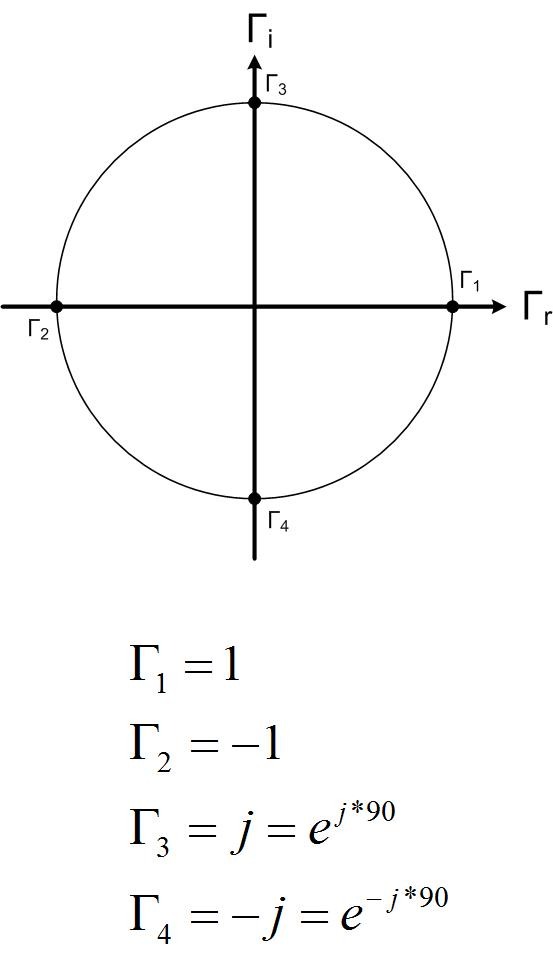
\includegraphics[scale=0.3]{../jpg/Smith_Chart_Reflection_Coefficient.jpg}
\end{center}
\caption{Examples of location of reflection coefficient on the Smith Chart.}
\label{scex}
\end{figure}


In Figure \ref{scswr1}, \ref{scswr}  circle and line shown represent all points on the Smith Chart that have constant magnitude or angle of the reflection coefficient. At high frequencies it is difficult to measure impedances directly, as it is difficult to measure (or sometimes even define) voltage and current. 
To measure impedances, engineers use Network Analyzer shown in Figure \ref{hp8510}.


\begin{figure}[htbp]
\begin{center}
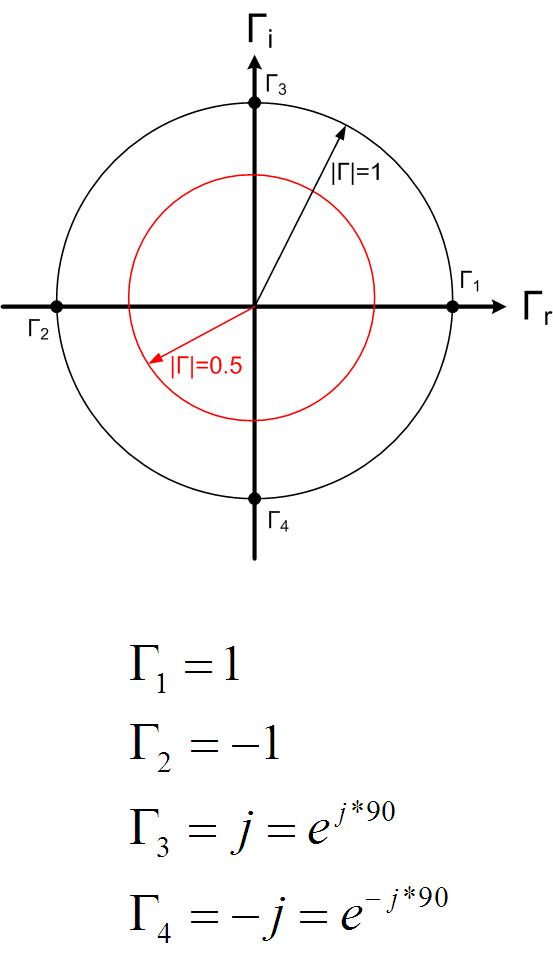
\includegraphics[scale=0.3]{../jpg/smithchartreflection.jpg}
\end{center}
\caption{Points of constant magnitude of the reflection coefficient. $ | \Gamma | $=0.5, $ | \Gamma |$=1}
\label{scswr1}
\end{figure}



\begin{figure}[htbp]
\begin{center}
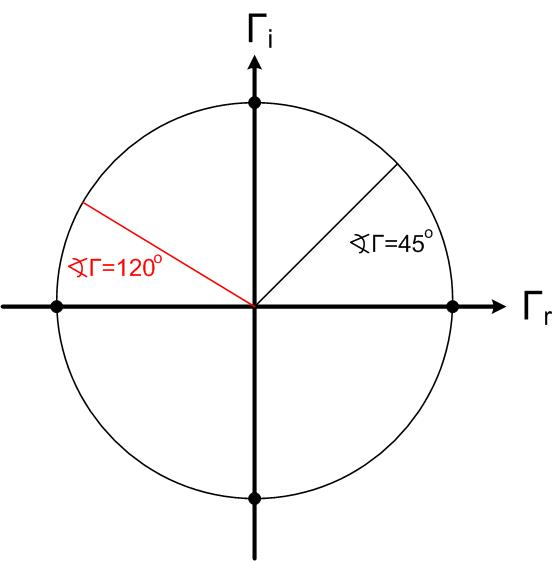
\includegraphics[scale=0.3]{../jpg/smithchartangle.jpg}
\end{center}
\caption{Points of constant phase of the reflection coefficient. $ < \Gamma =45^\circ$, $  <  \Gamma = 120^\circ$}
\label{scswr}
\end{figure}







\begin{figure}[htbp]
\begin{center}
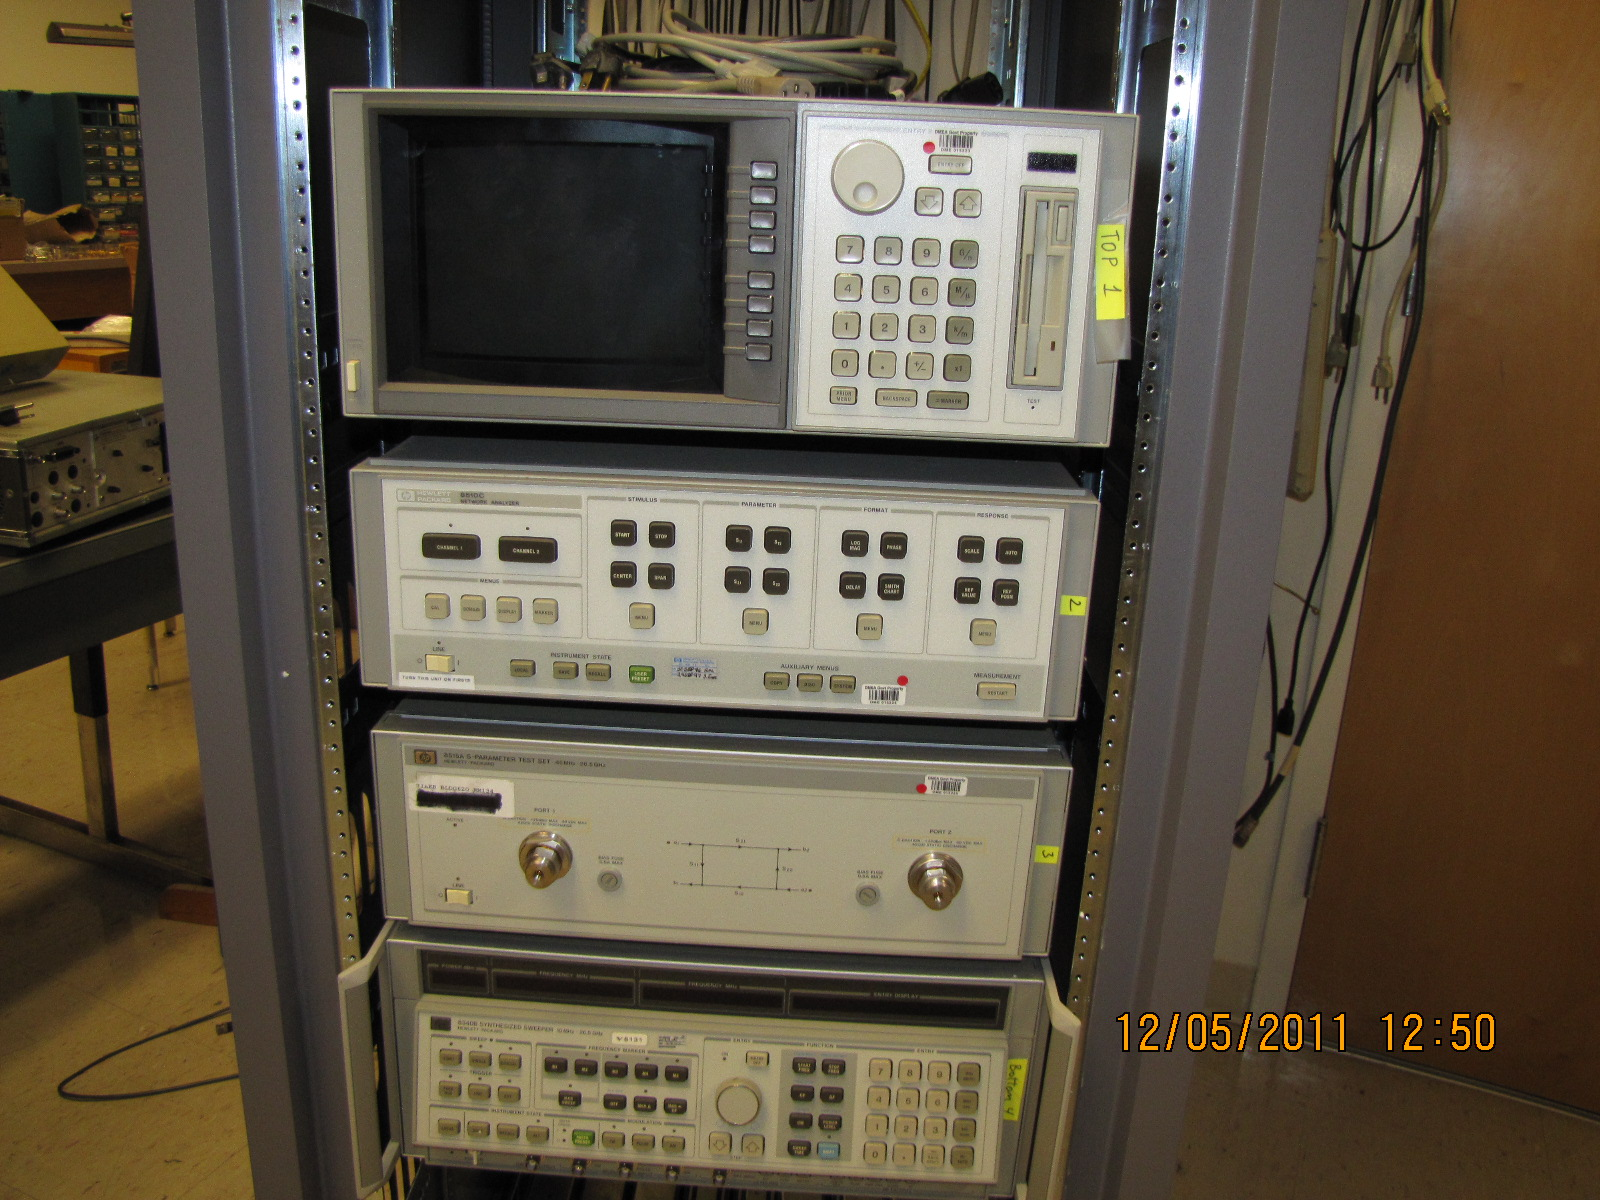
\includegraphics[scale=0.2]{../jpg/HP8510.jpg}
\end{center}
\caption{HP8510 Network Analyzer in Microwave Laboratory measures impedances up to 26.5GHz. This piece of equipment is on permanent loan curtesy of Defense Micro Electronic Activity (DMEA), Sacramento}
\label{hp8510}
\end{figure}


Since reflection coefficient and  impedance are related through Equation \ref{eqnreflectioncoefficient}, we can find impedance that corresponds to the  reflection coefficient, Equation \ref{eqnimpedancerc}. In other words, every point on the Smith Chart represents one reflection coefficient $\Gamma$ and one impedance $Z_L$. 



\begin{eqnarray}
\Gamma = \frac{Z_L-Z_\circ}{Z_L+Z_\circ} \label{eqnreflectioncoefficient} \\ \nonumber \\
z_L = \frac{Z_L}{Z_\circ} = \frac{ 1+ \Gamma}{1- \Gamma } \label{eqnimpedancerc}
\end{eqnarray}

Figures \ref{scresistance}- \ref{screactance}  shows circles on the Smith Chart that represent constant (normalized) reactances, and resistances. Figure \ref{scimpedance}, shows how to find  $z_L=1+j 1$. This impedance is at a point where the circle of constant resistance $r_L=1$ crosses the circle of constant reactance $x_L=1$.   Figure \ref{scgammafromZ} shows how to find the reflection coefficient if normalized load  impedance $z_L=1+j 1$ is given. Measure the distance bewteen the origin using the scale "Reflection Coefficient E or I"on the bottom of the Smith Chart to find the magnitude of the reflection coefficient. To find the angle of the reflection coefficient, we read the scale "Angle of Reflection Coefficient" on the perimeter of the Smith Chart, shown in green. The reflection coefficient is therefore $0.5 e^{j 62^o}$, which is close to the actual value   $0.5 e^{j 64^o}$. If you have done this using ruler and compass, and nicely sharpened pencil, you would get exactly the right answer. Try it out!

\begin{figure}[htbp]
\begin{center}
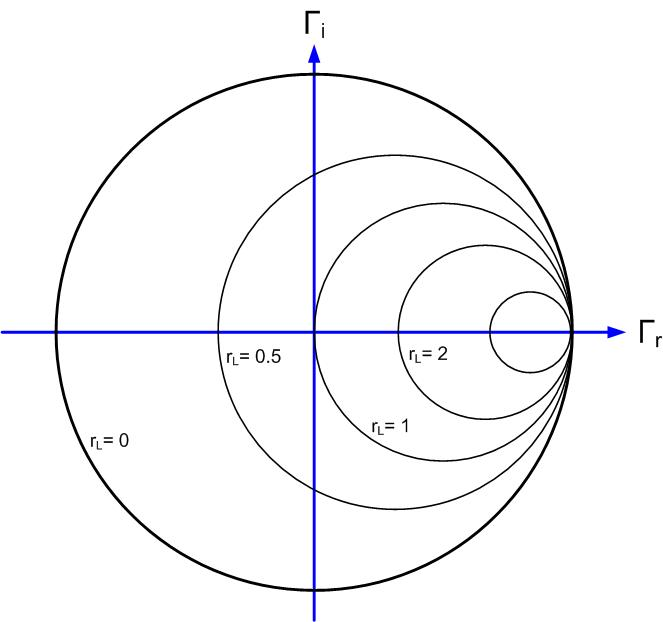
\includegraphics[scale=0.3]{/../jpg/smithchartreal.jpg}
\end{center}
\caption{All points on the circle have the constant real part of the impedance (resistance). Normalized resistance circles.}
\label{scresistance}
\end{figure}


\begin{figure}[htbp]
\begin{center}
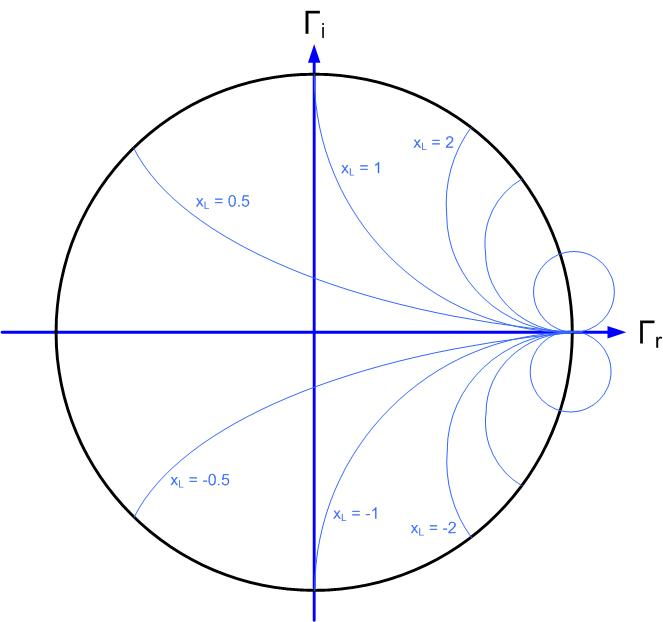
\includegraphics[scale=0.3]{../jpg/smithchartimaginary.jpg}
\end{center}
\caption{All points on the circle have the constant imaginary part of the impedance (reactance). Normalized reactance circles.}
\label{screactance}
\end{figure}



\begin{figure}[htbp]
\begin{center}
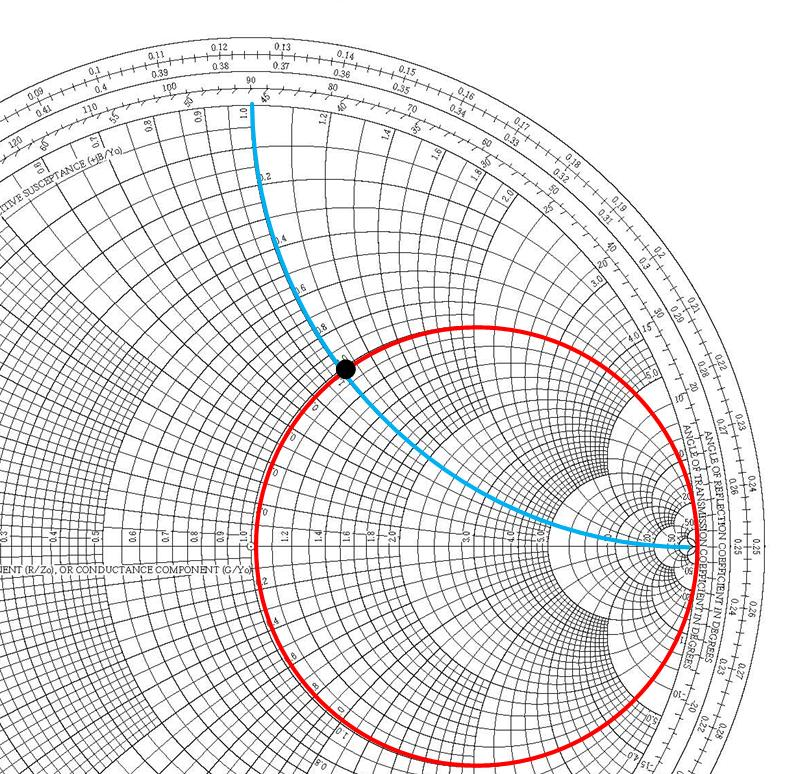
\includegraphics[scale=0.3]{../jpg/FindingImpedanceonSC.jpg}
\end{center}
\caption{Red circle that represents all points on Smith Chart with normalized resistance $r=1$ and blue circle that represents all points on Smith Chart with  normalized reactance $x=1$ cross at point where $Z_L=1+j 1$.}
\label{scimpedance}
\end{figure}

\begin{figure}[htbp]
\begin{center}
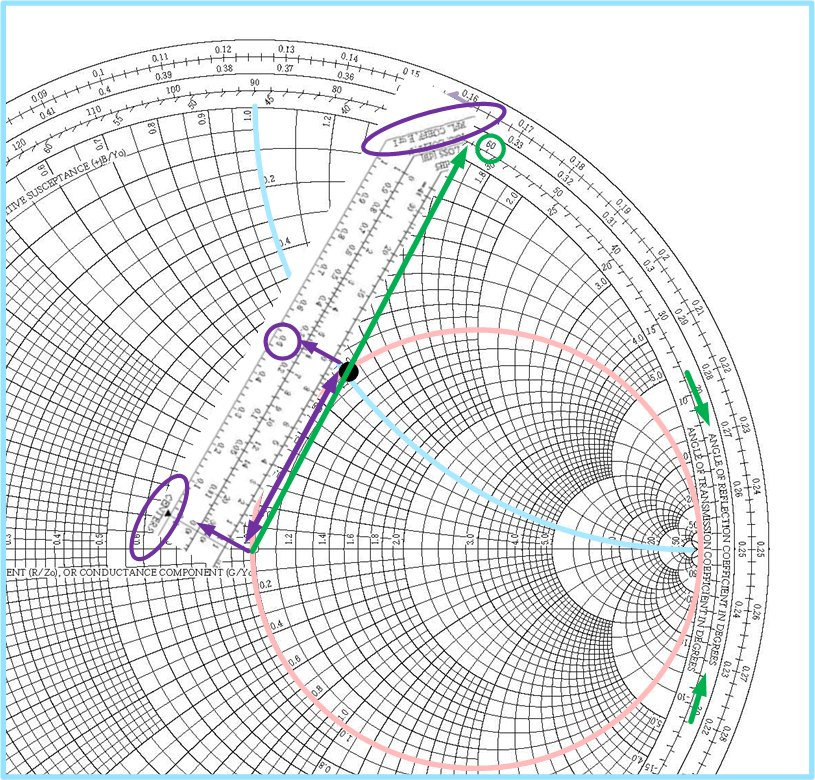
\includegraphics[scale=0.3]{../jpg/FindingGammaFromImpedanceonSC.jpg}
\end{center}
\caption{To find the magnitude of the reflection coefficient from impedance $Z_L=1+j 1$, we measure the distance bewteen the origin using the scale "Reflection Coefficient E or I"on the bottom of the Smith Chart. To find the angle of the reflection coefficient, we read the scale "Angle of Reflection Coefficient" on the perimeter of the Smith Chart.}
\label{scgammafromZ}
\end{figure}

\newpage

\subsection*{Brief review of impedance and admittance}

Impedance's real part is called resistance R, and imaginary part is called reactance X. Admittance's real part is called conductance, and imaginary part is called susceptance. It is easier to add impedances when elements are in series, and it is easier to add admittances when elements are in parallel, see Figure \ref{impadmtrans}, because we just add real and imaginary parts separately. This is the reason we have special Smith Chart shown in Figure \ref{scadmimp} that has both impedance and admittance circles on it.  This way, we can use Smith Chart to read off the values for equivalent impedance or admittance when we add impedances or admittances in parallel or series. This comes in handy for lumped-element impedance matching that we will talk about next.

\begin{figure}[htbp]
\begin{center}
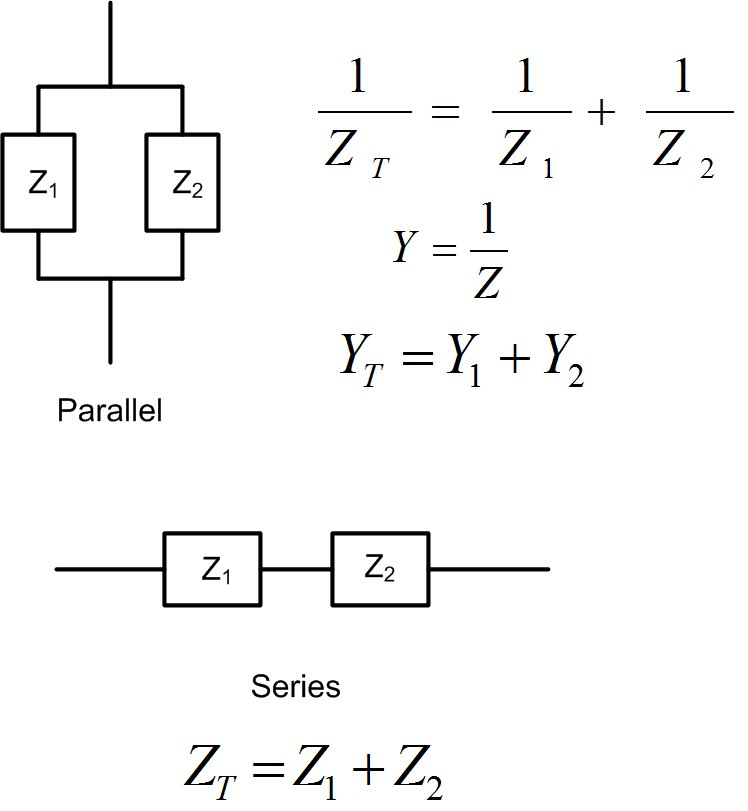
\includegraphics[scale=0.3]{../jpg/Impedance_Admittance.jpg}
\end{center}
\caption{It is easier to use admittance when the circuit elements are in parallel and impedance when the circuit elements are in series.}
\label{impadmtrans}
\end{figure}




\begin{figure}[htbp]
\begin{center}
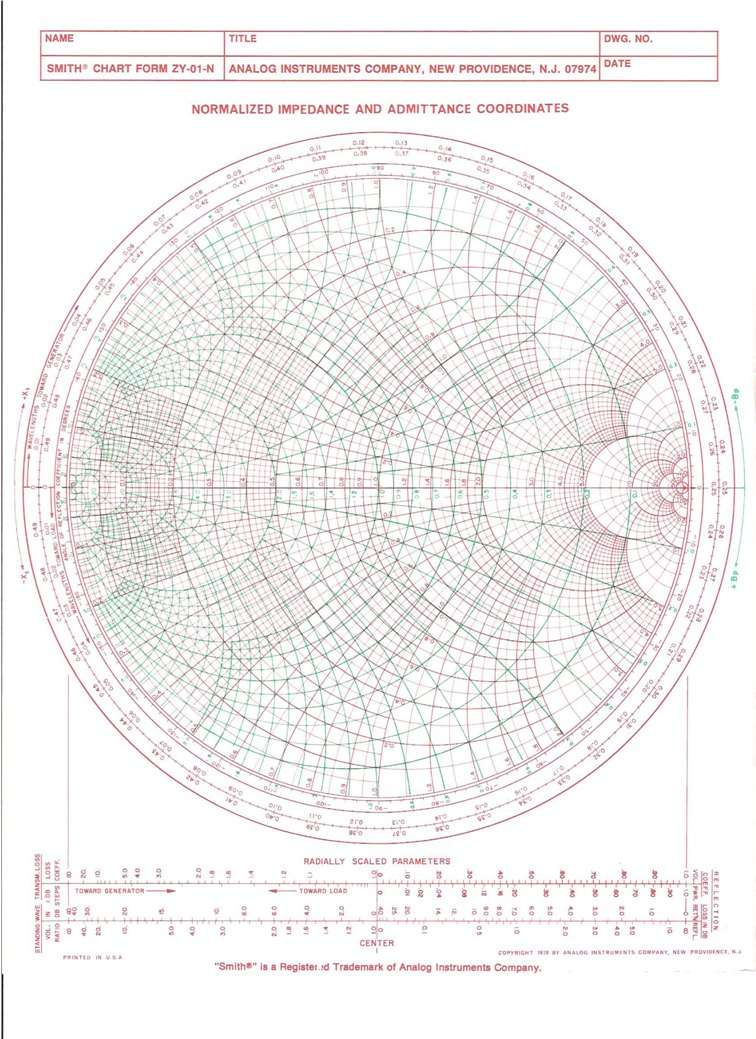
\includegraphics[scale=0.3]{../jpg/SCadmimp.jpg}
\end{center}
\caption{On Smith Chart impedances are shown in red, and admittances in green.}
\label{scadmimp}
\end{figure}



\end{document} 
